\documentclass{standalone}
\usepackage{tikz}
\usetikzlibrary{patterns, positioning}
\usepackage[sfdefault]{ClearSans} %% option 'sfdefault' activates Clear Sans as the default text font
\usepackage[T1]{fontenc}

\begin{document}
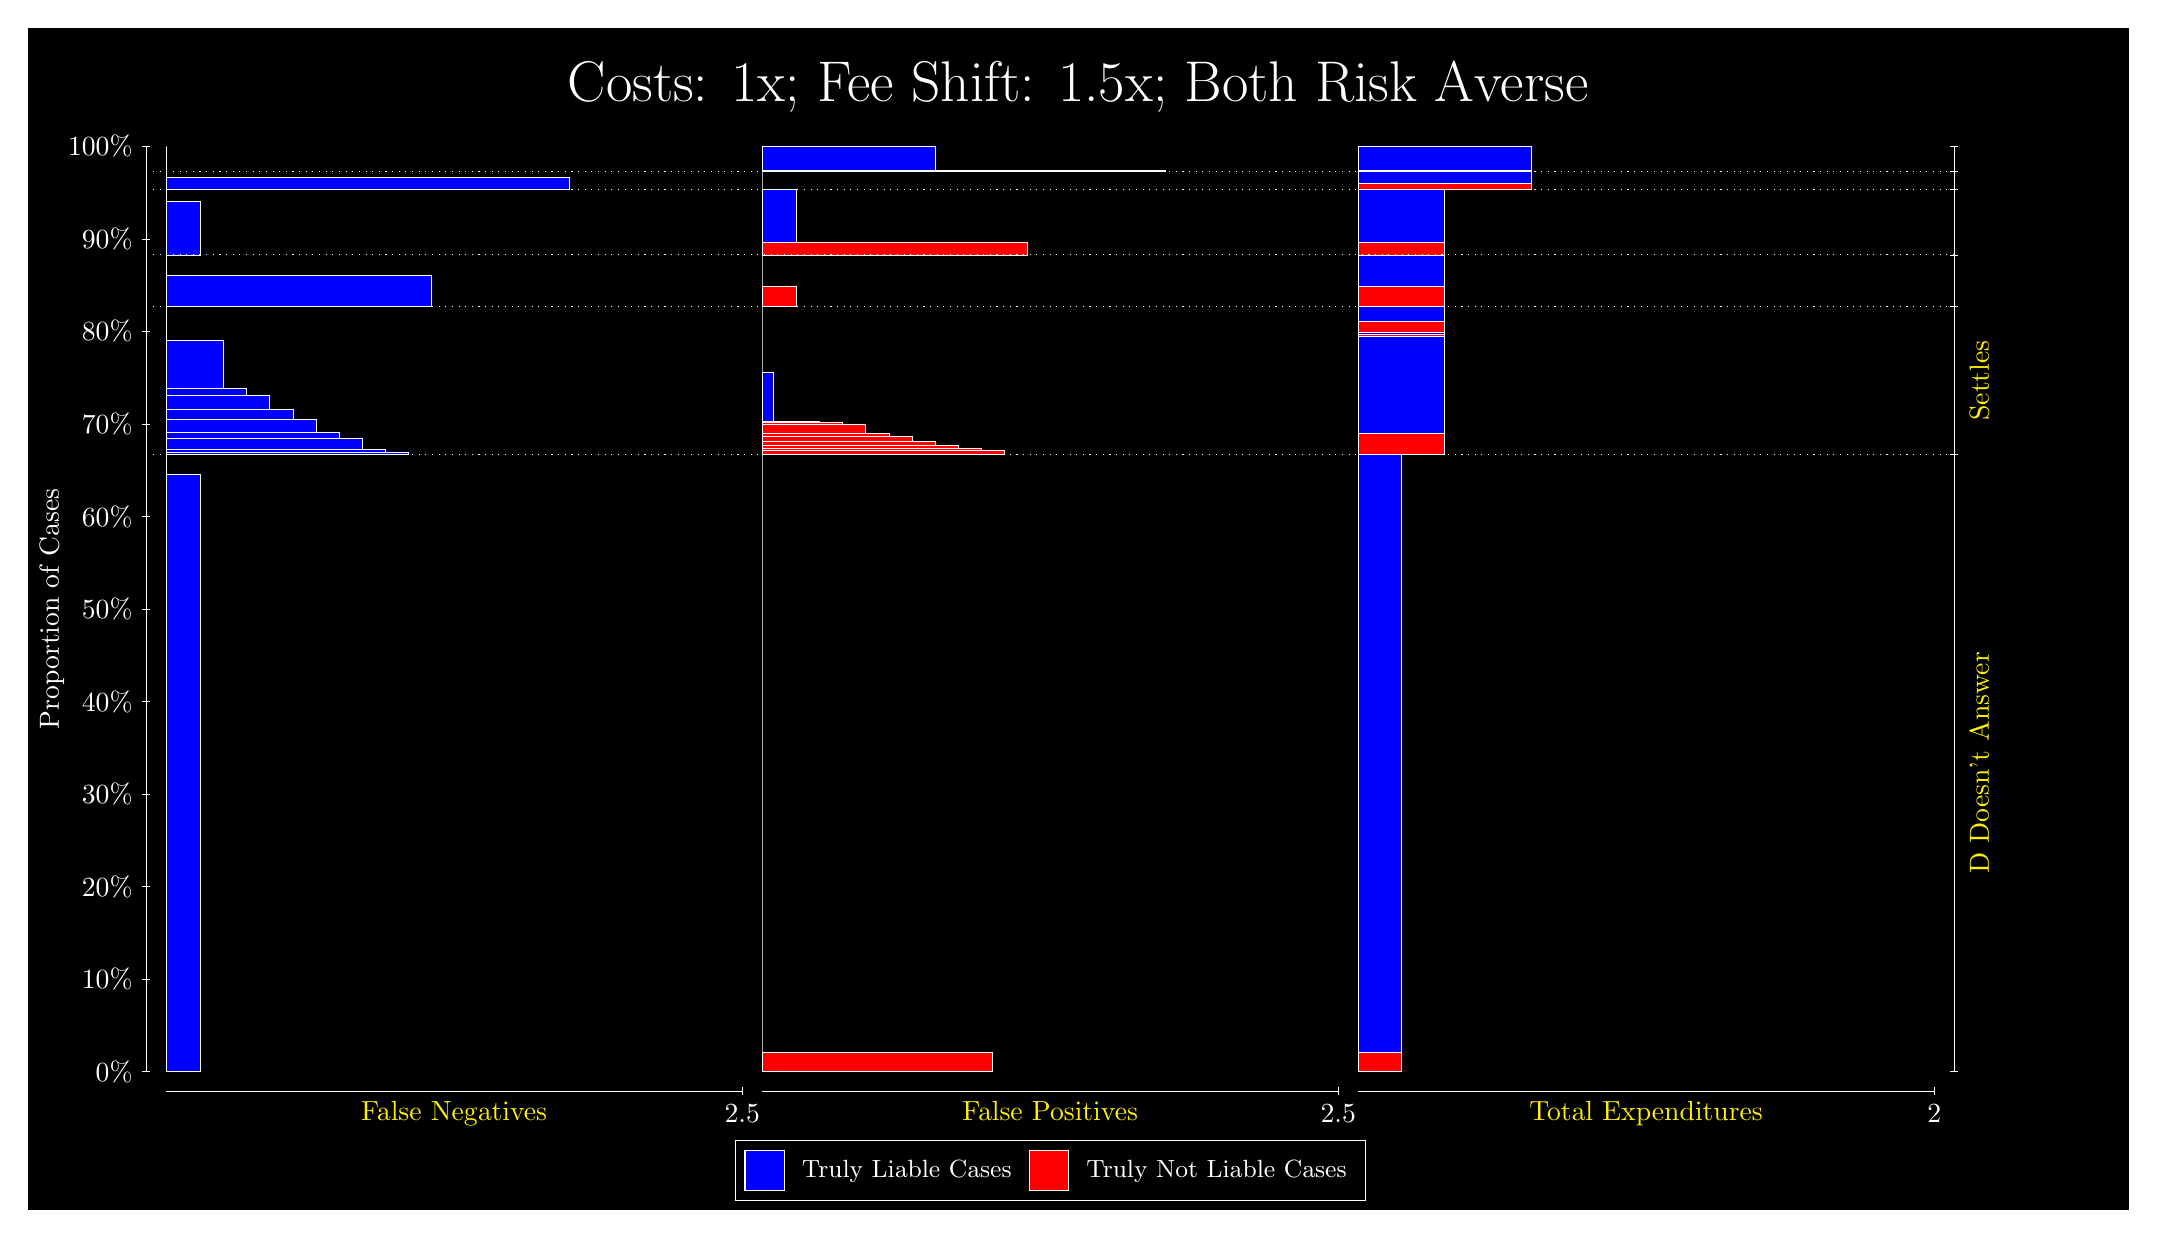
\begin{tikzpicture}
\draw[fill=black] (0,0) rectangle (26.667,15);
\draw[text=white] (0,13.5) rectangle (26.667,15) node[midway] {\huge Costs: 1x; Fee Shift: 1.5x; Both Risk Averse};
\draw[white, very thin] (1.5,1.75) -- (1.5,13.5);
\node[rotate=90, text=white, anchor=center] at (0.3, 7.625) {Proportion of Cases};
\draw[white, very thin] (1.45,1.75) -- (1.55,1.75);
\node[text=white, anchor=east] at (1.45, 1.75) {0\%};
\draw[white, very thin] (1.45,2.925) -- (1.55,2.925);
\node[text=white, anchor=east] at (1.45, 2.925) {10\%};
\draw[white, very thin] (1.45,4.1) -- (1.55,4.1);
\node[text=white, anchor=east] at (1.45, 4.1) {20\%};
\draw[white, very thin] (1.45,5.275) -- (1.55,5.275);
\node[text=white, anchor=east] at (1.45, 5.275) {30\%};
\draw[white, very thin] (1.45,6.45) -- (1.55,6.45);
\node[text=white, anchor=east] at (1.45, 6.45) {40\%};
\draw[white, very thin] (1.45,7.625) -- (1.55,7.625);
\node[text=white, anchor=east] at (1.45, 7.625) {50\%};
\draw[white, very thin] (1.45,8.8) -- (1.55,8.8);
\node[text=white, anchor=east] at (1.45, 8.8) {60\%};
\draw[white, very thin] (1.45,9.975) -- (1.55,9.975);
\node[text=white, anchor=east] at (1.45, 9.975) {70\%};
\draw[white, very thin] (1.45,11.15) -- (1.55,11.15);
\node[text=white, anchor=east] at (1.45, 11.15) {80\%};
\draw[white, very thin] (1.45,12.325) -- (1.55,12.325);
\node[text=white, anchor=east] at (1.45, 12.325) {90\%};
\draw[white, very thin] (1.45,13.5) -- (1.55,13.5);
\node[text=white, anchor=east] at (1.45, 13.5) {100\%};

\draw[white, very thin] (24.457,1.75) -- (24.457,13.5);
\draw[white, very thin] (24.407,1.75) -- (24.507,1.75);
\node[anchor=west] at (24.407, 1.75) {};
\draw[white, very thin] (24.407,9.5904) -- (24.507,9.5904);
\node[anchor=west] at (24.407, 9.5904) {};
\draw[white, very thin] (24.407,11.465) -- (24.507,11.465);
\node[anchor=west] at (24.407, 11.465) {};
\draw[white, very thin] (24.407,12.122) -- (24.507,12.122);
\node[anchor=west] at (24.407, 12.122) {};
\draw[white, very thin] (24.407,12.952) -- (24.507,12.952);
\node[anchor=west] at (24.407, 12.952) {};
\draw[white, very thin] (24.407,13.177) -- (24.507,13.177);
\node[anchor=west] at (24.407, 13.177) {};
\draw[white, very thin] (24.407,13.5) -- (24.507,13.5);
\node[anchor=west] at (24.407, 13.5) {};

\draw[white, very thin, fill=blue] (1.75,1.75) rectangle (2.1891,9.341);
\draw[white, very thin, fill=red] (1.75,9.341) rectangle (1.75,9.5904);
\draw[white, very thin, fill=blue] (1.75,9.5904) rectangle (4.8239,9.6183);
\draw[white, very thin, fill=blue] (1.75,9.6183) rectangle (4.5312,9.6576);
\draw[white, very thin, fill=blue] (1.75,9.6576) rectangle (4.2384,9.7933);
\draw[white, very thin, fill=blue] (1.75,9.7933) rectangle (3.9457,9.87);
\draw[white, very thin, fill=blue] (1.75,9.87) rectangle (3.6529,10.028);
\draw[white, very thin, fill=blue] (1.75,10.028) rectangle (3.3602,10.158);
\draw[white, very thin, fill=blue] (1.75,10.158) rectangle (3.0674,10.332);
\draw[white, very thin, fill=blue] (1.75,10.332) rectangle (2.7746,10.423);
\draw[white, very thin, fill=blue] (1.75,10.423) rectangle (2.4819,11.043);
\draw[white, very thin, fill=red] (1.75,11.043) rectangle (1.75,11.465);
\draw[white, very thin, fill=blue] (1.75,11.465) rectangle (5.1167,11.863);
\draw[white, very thin, fill=red] (1.75,11.863) rectangle (1.75,12.122);
\draw[white, very thin, fill=blue] (1.75,12.122) rectangle (2.1891,12.797);
\draw[white, very thin, fill=red] (1.75,12.797) rectangle (1.75,12.952);
\draw[white, very thin, fill=blue] (1.75,12.952) rectangle (6.8732,13.103);
\draw[white, very thin, fill=red] (1.75,13.103) rectangle (1.75,13.177);
\draw[white, very thin, fill=red] (1.75,13.177) rectangle (1.75,13.194);
\draw[white, very thin, fill=blue] (1.75,13.194) rectangle (1.75,13.5);
\draw[white, very thin, fill=red] (9.3189,1.75) rectangle (12.246,1.9994);
\draw[white, very thin, fill=blue] (9.3189,1.9994) rectangle (9.3189,9.5904);
\draw[white, very thin, fill=red] (9.3189,9.5904) rectangle (12.393,9.636);
\draw[white, very thin, fill=red] (9.3189,9.636) rectangle (12.1,9.6606);
\draw[white, very thin, fill=red] (9.3189,9.6606) rectangle (11.807,9.7048);
\draw[white, very thin, fill=red] (9.3189,9.7048) rectangle (11.515,9.752);
\draw[white, very thin, fill=red] (9.3189,9.752) rectangle (11.222,9.8127);
\draw[white, very thin, fill=red] (9.3189,9.8127) rectangle (10.929,9.8524);
\draw[white, very thin, fill=red] (9.3189,9.8524) rectangle (10.929,9.8562);
\draw[white, very thin, fill=red] (9.3189,9.8562) rectangle (10.636,9.965);
\draw[white, very thin, fill=red] (9.3189,9.965) rectangle (10.344,9.9931);
\draw[white, very thin, fill=red] (9.3189,9.9931) rectangle (10.051,10.011);
\draw[white, very thin, fill=blue] (9.3189,10.011) rectangle (9.4652,10.632);
\draw[white, very thin, fill=blue] (9.3189,10.632) rectangle (9.3189,11.465);
\draw[white, very thin, fill=red] (9.3189,11.465) rectangle (9.758,11.723);
\draw[white, very thin, fill=blue] (9.3189,11.723) rectangle (9.3189,12.122);
\draw[white, very thin, fill=red] (9.3189,12.122) rectangle (12.686,12.277);
\draw[white, very thin, fill=blue] (9.3189,12.277) rectangle (9.758,12.952);
\draw[white, very thin, fill=red] (9.3189,12.952) rectangle (9.3189,13.026);
\draw[white, very thin, fill=blue] (9.3189,13.026) rectangle (9.3189,13.177);
\draw[white, very thin, fill=red] (9.3189,13.177) rectangle (14.442,13.194);
\draw[white, very thin, fill=blue] (9.3189,13.194) rectangle (11.515,13.5);
\draw[white, very thin, fill=red] (16.888,1.75) rectangle (17.437,1.9994);
\draw[white, very thin, fill=blue] (16.888,1.9994) rectangle (17.437,9.5904);
\draw[white, very thin, fill=red] (16.888,9.5904) rectangle (17.986,9.8524);
\draw[white, very thin, fill=blue] (16.888,9.8524) rectangle (17.986,11.093);
\draw[white, very thin, fill=red] (16.888,11.093) rectangle (17.986,11.111);
\draw[white, very thin, fill=blue] (16.888,11.111) rectangle (17.986,11.139);
\draw[white, very thin, fill=red] (16.888,11.139) rectangle (17.986,11.28);
\draw[white, very thin, fill=blue] (16.888,11.28) rectangle (17.986,11.465);
\draw[white, very thin, fill=red] (16.888,11.465) rectangle (17.986,11.723);
\draw[white, very thin, fill=blue] (16.888,11.723) rectangle (17.986,12.122);
\draw[white, very thin, fill=red] (16.888,12.122) rectangle (17.986,12.277);
\draw[white, very thin, fill=blue] (16.888,12.277) rectangle (17.986,12.952);
\draw[white, very thin, fill=red] (16.888,12.952) rectangle (19.083,13.026);
\draw[white, very thin, fill=blue] (16.888,13.026) rectangle (19.083,13.177);
\draw[white, very thin, fill=red] (16.888,13.177) rectangle (19.083,13.194);
\draw[white, very thin, fill=blue] (16.888,13.194) rectangle (19.083,13.5);
\draw[white, dotted] (1.5,9.5904) -- (24.457,9.5904);
\draw[white, dotted] (1.5,11.465) -- (24.457,11.465);
\draw[white, dotted] (1.5,12.122) -- (24.457,12.122);
\draw[white, dotted] (1.5,12.952) -- (24.457,12.952);
\draw[white, dotted] (1.5,13.177) -- (24.457,13.177);
\draw[white, very thin] (1.75,1.5) -- (9.0689,1.5);
\node[text=yellow, anchor=north] at (5.4094, 1.5) {False Negatives};
\draw[white, very thin] (9.0689,1.45) -- (9.0689,1.55);
\node[text=white, anchor=north] at (9.0689, 1.45) {2.5};

\draw[white, very thin] (9.3189,1.5) -- (16.638,1.5);
\node[text=yellow, anchor=north] at (12.978, 1.5) {False Positives};
\draw[white, very thin] (16.638,1.45) -- (16.638,1.55);
\node[text=white, anchor=north] at (16.638, 1.45) {2.5};

\draw[white, very thin] (16.888,1.5) -- (24.207,1.5);
\node[text=yellow, anchor=north] at (20.547, 1.5) {Total Expenditures};
\draw[white, very thin] (24.207,1.45) -- (24.207,1.55);
\node[text=white, anchor=north] at (24.207, 1.45) {2};

\node[text=yellow, centered, rotate=90] at (24.777, 5.6702) {D Doesn't Answer};
\node[text=yellow, centered, rotate=90] at (24.777, 10.527) {Settles};





\draw (12.978300999999998,1.5) node[draw=none] (baseCoordinate) {};
\begin{scope}[align=center]
        \matrix[scale=0.5, draw=white, below=0.5cm of baseCoordinate, nodes={draw}, column sep=0.1cm]{
            \node[rectangle, draw, minimum width=0.5cm, minimum height=0.5cm, fill=blue] {}; &
            \node[draw=none, font=\small, text=white] (B) {Truly Liable Cases}; &
            \node[rectangle, draw, minimum width=0.5cm, minimum height=0.5cm, fill=red] {}; &
            \node[draw=none, font=\small, text=white] (B) {Truly Not Liable Cases}; \\
            };
\end{scope}

\end{tikzpicture}
\end{document}